\documentclass[12pt,fleqn]{article}
\usepackage{booktabs}
\usepackage{tabularx}
\usepackage{hyperref}
\usepackage{float}
\hypersetup{
    colorlinks,
    citecolor=black,
    filecolor=black,
    linkcolor=black,
    urlcolor=blue
}
\usepackage[round]{natbib}
\usepackage{graphicx}
\usepackage{paralist}
\usepackage{amsfonts}
\usepackage{vhistory}
\usepackage{tcolorbox}


\oddsidemargin 0mm
\evensidemargin 0mm
\textwidth 160mm
\textheight 200mm
\renewcommand\baselinestretch{1.0}
\usepackage{fancyhdr}
\fancyhead[L]{November 29, 2017}
\fancyhead[C]{SE 3XA3: Test Plan}
\fancyhead[R]{AKT}
\pagestyle{fancy}

\pagenumbering{arabic}

\newcounter{stepnum}

\title{Group 29 (AKT)\\ Test Plan}
\author{
Alex Trudeau\\
	\texttt{400030148}
\and
Kathryn Kodama\\
  	\texttt{400013582}
\and
Tommy Tran\\
	\texttt{001150067}
}
\date{\today\\Version 2.0}
\begin{document}

\maketitle



\pagebreak
\tableofcontents


\listoftables

\begin{table}[ht]
\caption{\bf Revision History}
\begin{tabularx}{\textwidth}{p{3cm}p{2cm}X}
\toprule {\bf Version} & {\bf Date} & {\bf Notes}\\
\midrule
1.0 & 18/10/17 & Created Document\\
1.1 & 24/10/17 & Updated  content and formatting\\
1.2 & 26/10/17 & Updated content\\
1.3 & 27/10/17 & Finalized content for Rev.0 \\
2.0 & 20/11/17 & Started Rev.1 \\
\bottomrule
\end{tabularx}
\textbf{*list of figures is not applicable to this document as of version 1.3}
\end{table}



\clearpage



\section {General Information}

\subsection {Purpose}
The purpose of this test plan is to verify that the program works as intended and was implemented correctly with the utmost confidence.

\subsection {Scope}
This test plan provides the basis for testing the Reddit-Clone program's functionality and that it properly mimics the functionality of the original open source project Reddit.  The program allows for users to post, discuss, and curate user created content.

The testing of Reddit-Clone means to cover the entirety of the project through black box, white box, manual, and automated tests.  This document is an outline of the testing methods including the testing tools to be utilized.

\subsection {Acronyms, Abbreviations, and Symbols}

\begin{table}[ht]
\caption{\textbf{Table of Abbreviations}} \label{Abbreviations}
\begin{tabularx}{\textwidth}{p{3cm}X}
\toprule
\textbf{Abbreviation} & \textbf{Definition} \\
\midrule
AKT & Alex, Kathryn, Tommy; also the team name (see Definitions table)\\
PoC & Proof of concept, project as of October 16, 2017\\
DevPlan & Development Plan document \\
UI & User Interaction \\
\bottomrule
\end{tabularx}
\end{table}

\begin{table}[ht]
\caption{\textbf{Table of Definitions}} \label{Definitions}
\begin{tabularx}{\textwidth}{p{3cm}X}
\toprule
\textbf{Term} & \textbf{Definition}\\
\midrule
AKT & The developer team for Reddit-Clone\\
Black Box Testing & A testing method where the code is tested without knowledge of the internal structure \\
Comment & An authenticated user's text response to another user's post or comment \\
Down-dote & A term for "disliking" a post/comment on Reddit-Clone. \\
Dynamic Testing & A type of testing where the software is tested based on specific input values to see if it matches the expected output values \\
GUI & Graphic User Interface \\ 
Manual Testing & A type of testing where the tester plays the role of the end user and uses most of the application's features to ensure correct behaviour \\
Post & A submission by an authenticated user that contains text and/or media attachments \\
Reddit & The original Reddit open source projected to be recreated (\url{http://www.reddit.com})\\
Reddit-Clone & The project being created.\\
Subreddit & A page containing the posts of a certain topic \\
System Testing & A type of testing where the entire software and integration is tested. System testing is a subset of black box testing.\\
Up-vote & A term for "liking" a post/comment on Reddit-Clone.  \\
White Box Testing & A type of testing where the software is tested with knowledge of the inner workings of the code \\
\bottomrule
\end{tabularx}
\end{table}	

\pagebreak
\section {Plan}
This section provides information on the Reddit-Clone project and the software testing plan. This plan is based off of the main functionality that exists as of the PoC as well as any additional functions outlined in the DevPlan.

\subsection {Software Description}
Reddit-Clone will allow authenticated users create posts, subreddits and comments as well as curate others' content through up-votes and down-votes.  The program is implemented in JavaScript with Angular 4 and Ionic 2 framework.

\subsection {Test Team}
The testing team for Reddit-Clone are all members of the AKT Development team: Alex Trudeau, Kathryn Kodama, Tommy Tran.  The lead tester will be Tommy Tran.

\subsection {Tools Used for Testing}
The dynamic testing will utilize the following tools.  Jasmine with Karma framework and Angular 4 testing packages will be used to dynamically test the JavaScript functionality of this project.  Through the use of Jasmine the testing team will carry out unit tests and end to end testing.

The HTML/CSS testing will be tested through static testing and observation on Unix, Windows, iOS, and Android environments.

\subsection {Testing Schedule}

Refer to the \href{https://gitlab.cas.mcmaster.ca/trudeaua/reddit-clone}{Gantt Chart} located in the project GitLab for the testing schema.   Testing is divided into the following categories within the Gantt chart: Account Management, Content Management, Navigation Methods.  Each testing category is assigned to a different member of the AKT development team and associated with a start date and end date.

\begin{table}[ht]
\caption{\bf Testing Schedule (as outlined in the Gantt Chart)}
\begin{tabularx}{\textwidth}{p{3cm}p{2cm}X}
\toprule {\bf Category} & {\bf Group Member} & {\bf Completion Date}\\
\midrule
Set up testing framework & Kathryn Kodama; Tommy Tran & 5/11/2017 \\
Account Management & Alex Trudeau & 10/11/2017\\
Content Management & Tommy Tran & 12/11/2017 \\
Navigation Methods & Kathryn Kodama & 11/11/2017\\ 
\bottomrule
\end{tabularx}
\end{table}


\pagebreak

% Authentication Methods, Account Management, Content Management, Navigation Methods, 
\section{Traceability Matrix}
Please view the requirements specification document to view the functional and non-functional requirements located in the traceability matrix below.  The tests detailed our outlined in the sections below.\\
\newline
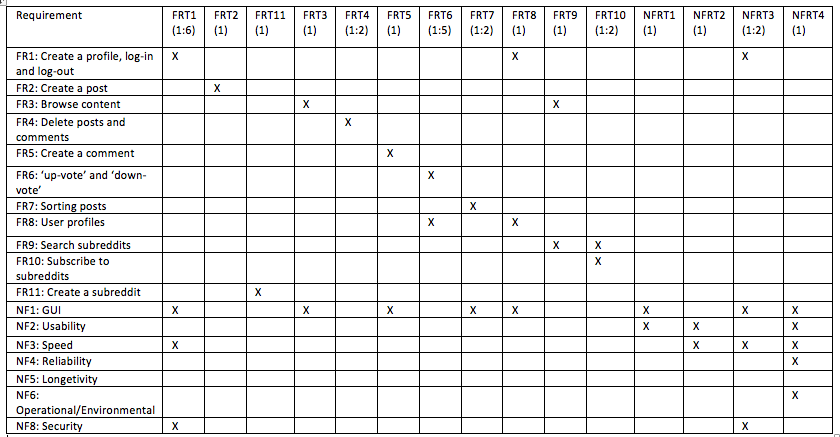
\includegraphics[scale=0.55]{matrix.png}

\pagebreak
\section{System Testing}
\subsection{Tests for Functional Requirements}
\subsubsection{Account Management}

\textbf{User account creation (valid inputs)}
\begin{tcolorbox}
\textbf{Test ID:} FRT1-1\\
\textbf{Type:} Functional, Dynamic, Manual\\
\textbf{Initial State:} Not authenticated, on home page\\
\textbf{Input:} Enter valid username, email and password\\
\textbf{Output:} Email sent to inputted email(user cannot log in yet). \\
\textbf{How the test will be performed:} Tester will sign up and after successful sign up, check that an email was received. Database will also be verified for successful user creation.
\end{tcolorbox}

\textbf{\\User account creation (invalid inputs)}
\begin{tcolorbox}
\textbf{Test ID:} FRT1-2\\
\textbf{Type:} Functional, Dynamic, Manual\\
\textbf{Initial State:} Not authenticated, on home page\\
\textbf{Input:} Enter invalid or already registered username/email\\
\textbf{Output:} Error message shown to user.  This test generates an exception.\\
\textbf{How the test will be performed:} Tester will attempt sign up with an invalid or already used username or email.
\end{tcolorbox}

\textbf{\\Verify user account}
\begin{tcolorbox}
\textbf{Test ID:} FRT1-3\\
\textbf{Type:} Functional, Dynamic, Manual\\
\textbf{Initial State:} After successful user account creation\\
\textbf{Input:} Open verification link in email \\
\textbf{Output:} Success message \\
\textbf{How the test will be performed:} Tester will check account email and open the verification link
\end{tcolorbox}

\newpage



\textbf{\\Log in}
\begin{tcolorbox}
\textbf{Test ID:} FRT1-4\\
\textbf{Type:} Functional, Dynamic, Manual\\
\textbf{Initial State:} Prompted to log in\\
\textbf{Input:} Enter user information from previously created account\\
\textbf{Output:} Successful or failed authentication
\textbf{How the test will be performed:} The user will log into the application with an email not associated with any account (authentication fails). Then the user will log in with a previously created user account (authentication succeeds).
\end{tcolorbox}

\textbf{\\Log in (unverified)}
\begin{tcolorbox}
\textbf{Test ID:} FRT1-5\\
\textbf{Type:} Functional, Dynamic, Manual\\
\textbf{Initial State:} User prompted to log in\\
\textbf{Input:} The user will enter user information from previously created account.\\
\textbf{Output:} An error message should appear notifying the user to verify their account via their email.
\textbf{How the test will be performed:} The user will log in with a previously created user account. The authentication succeeds but will then prompt the user to check their email to verify their account. 
\end{tcolorbox}

\textbf{\\Log out}
\begin{tcolorbox}
\textbf{Test ID:} FRT1-6\\
\textbf{Type:} Functional, Dynamic, Manual\\
\textbf{Initial State:} Authenticated, viewing homepage\\
\textbf{Input:} Log out button selected\\
\textbf{Output:} Log in/Sign Up button shown on homepage\\
\textbf{How the test will be performed:} Log out and then confirm that authenticated user privileges were lost.
\end{tcolorbox}

\subsubsection{Content Management}

\textbf{Post creation}
\begin{tcolorbox}
\textbf{Test ID:} FRT2-1\\
\textbf{Type:} Functional, Dynamic, Manual\\
\textbf{Initial State:} Authenticated, create post modal opened\\
\textbf{Input:} Test post parameters\\
\textbf{Output:} Check post shows in subreddit\\
\textbf{How the test will be performed:} Authenticated account will create a test post and verify that a post shows in the posted subreddit afterwards
\end{tcolorbox}

\textbf{\\Subreddit creation}
\begin{tcolorbox}
\textbf{Test ID:} FRT11-1\\ % FR 11 users can create subreddits 
\textbf{Type:} Functional, Dynamic, Manual\\
\textbf{Initial State:} Authenticated, create subreddit modal opened\\
\textbf{Input:} Test subreddit name and description\\
\textbf{Output:} Subreddit created\\
\textbf{How the test will be performed:} Authenticated account will create a test subreddit and verify that the subreddit exists and was added to the subreddit navigation list
\end{tcolorbox}

\newpage

\textbf{\\Content browsing}
\begin{tcolorbox}
\textbf{Test ID:} FRT3-1\\
\textbf{Type:} Functional, Dynamic, Manual\\
\textbf{Initial State:} Authenticated\\
\textbf{Input:} View homepage and then select a subreddit\\
\textbf{Output:} Show posts from a variety of subreddits on homepage, show posts from specific subreddit when selected\\
\textbf{How the test will be performed:} Tester will manually view and verify that posts from multiple subreddits show on the homepage and when a subreddit is selected, posts from only that specific subreddit is shown
\end{tcolorbox}

\textbf{\\Delete posts}
\begin{tcolorbox}
\textbf{Test ID:} FRT4-1\\
\textbf{Type:} Structural, Dynamic, Automated\\
\textbf{Initial State:} Authenticated\\
\textbf{Input:} Send delete request for test post to database\\
\textbf{Output:} Test post deleted\\
\textbf{How the test will be performed:} Authenticated test account will send a request to delete a post and then verify that the post has been successfully deleted.
\end{tcolorbox}

\textbf{\\Delete comment}
\begin{tcolorbox}
\textbf{Test ID:} FRT4-2\\
\textbf{Type:} Structural, Dynamic, Automated\\
\textbf{Initial State:} Authenticated\\
\textbf{Input:} Send delete request for test comment to database\\
\textbf{Output:} Test comment deleted\\
\textbf{How the test will be performed:} Authenticated test account will send a request to delete a comment and then verify that the comment has been successfully deleted.
\end{tcolorbox}

\textbf{\\Create comment}
\begin{tcolorbox}
\textbf{Test ID:} FRT5-1\\
\textbf{Type:} Structural, Dynamic, Automated\\
\textbf{Initial State:} Authenticated\\
\textbf{Input:} Send a request to create a test comment to database\\
\textbf{Output:} Test comment created\\
\textbf{How the test will be performed:} Authenticated test account will send a request to create a comment and then verify that the comment has been successfully created.
\end{tcolorbox}

\textbf{\\Up-voting a post}
\begin{tcolorbox}
\textbf{Test ID:} FRT6-1\\
\textbf{Type:} Structural, Dynamic, Automated\\
\textbf{Initial State:} Authenticated\\
\textbf{Input:} Send a request to upvote test post to database\\
\textbf{Output:} Test post points increased\\
\textbf{How the test will be performed:} Authenticated test account will send a request to upvote a post and then verify that the post points has been successfully incremented.
\end{tcolorbox}

\textbf{\\Down-voting a post}
\begin{tcolorbox}
\textbf{Test ID:} FRT6-2\\
\textbf{Type:} Structural, Dynamic, Automated\\
\textbf{Initial State:} Authenticated\\
\textbf{Input:} Send a request to downvote a test post to database\\
\textbf{Output:} Test post points decreased\\
\textbf{How the test will be performed:} Authenticated test account will send a request to downvote a post and then verify that the post points has been successfully decremented.
\end{tcolorbox}

\textbf{\\Up-voting a comment}
\begin{tcolorbox}
\textbf{Test ID:} FRT6-3\\
\textbf{Type:} Structural, Dynamic, Automated\\
\textbf{Initial State:} Authenticated\\
\textbf{Input:} Send a request to upvote test comment to database\\
\textbf{Output:} Test comment points increased\\
\textbf{How the test will be performed:} Authenticated test account will send a request to upvote a comment and then verify that the comment points has been successfully incremented.
\end{tcolorbox}

\textbf{\\Down-voting a comment}
\begin{tcolorbox}
\textbf{Test ID:} FRT6-4\\
\textbf{Type:} Structural, Dynamic, Automated\\
\textbf{Initial State:} Authenticated\\
\textbf{Input:} Send a request to downvote a test comment to database\\
\textbf{Output:} Test comment points decreased\\
\textbf{How the test will be performed:} Authenticated test account will send a request to downvote a comment and then verify that the comment points has been successfully decremented.
\end{tcolorbox}

\textbf{\\User karma points}
\begin{tcolorbox}
\textbf{Test ID:} FRT6-5\\ % Need to modify FR6(modifications karma to user profile)
\textbf{Type:} Structural, Dynamic, Manual\\
\textbf{Initial State:} Authenticated\\
\textbf{Input:} Upvote/downvote a user's post/comment, select the user's name to open user profile  \\
\textbf{Output:} User profile modal opened(karma points should have changed)\\
\textbf{How the test will be performed:} Tester will upvote or downvote a user's post or comment and then select the user to view their information. The karma points should then be verified to change according to the upvote or downvote.
\end{tcolorbox}

\textbf{\\Sorting posts (Home page)}
\begin{tcolorbox}
\textbf{Test ID:} FRT7-1\\
\textbf{Type:} Functional, Dynamic, Manual\\
\textbf{Initial State:} Authenticated, on home page\\
\textbf{Input:} Select all three different sorting options: Hot, New and Top \\
\textbf{Output:} All posts sorted according to selection\\
\textbf{How the test will be performed:} Tester will select different sorting option and verify that sorting works. Hot shows more recently popular posts, New shows newest posts and Top shows posts with highest karma points.
\end{tcolorbox}

\textbf{\\Sorting posts (Subreddit)}
\begin{tcolorbox}
\textbf{Test ID:} FRT7-2\\
\textbf{Type:} Functional, Dynamic, Manual\\
\textbf{Initial State:} Authenticated, on test subreddit\\
\textbf{Input:} Select all three different sorting options: Hot, New and Top \\
\textbf{Output:} All posts sorted according to selection\\
\textbf{How the test will be performed:} Tester will select different sorting option on the test subreddit and verify that sorting works. Hot shows more recently popular posts, New shows newest posts and Top shows posts with highest karma points.
\end{tcolorbox}

\subsubsection{Navigation Methods}

\textbf{\\View user profile}
\begin{tcolorbox}
\textbf{Test ID:} FRT8-1\\
\textbf{Type:} Functional, Dynamic, Manual\\
\textbf{Initial State:} Application active \\
\textbf{Input:} Select user to open user profile  \\
\textbf{Output:} User profile modal opened\\
\textbf{How the test will be performed:} Tester will select a user to view their information and verify that all of the information is correct with the database.
\end{tcolorbox}

\textbf{\\Edit user profile picture}
\begin{tcolorbox}
\textbf{Test ID:} FRT8-2\\
\textbf{Type:} Functional, Dynamic, Manual\\
\textbf{Initial State:} Application active \\
\textbf{Input:} Select update photo and add link url, click "Submit"  \\
\textbf{Output:} User profile picture changed\\
\textbf{How the test will be performed:} Tester will select a user to view their information and change the profile photo.  The user will log in and out to ensure the new profile picture has been saved to their account.
\end{tcolorbox}

\textbf{\\View subreddit}
\begin{tcolorbox}
\textbf{Test ID:} FRT9-1\\ % Need to add new functional requirement: allow users to view subreddits
\textbf{Type:} Functional, Dynamic, Manual\\
\textbf{Initial State:} Application active \\
\textbf{Input:} Select a test subreddit or use subreddit navigation \\
\textbf{Output:} Test subreddit displayed\\
\textbf{How the test will be performed:} Tester will have the application opened and select a subreddit. The subreddit should then be displayed
\end{tcolorbox}

\newpage

\textbf{\\Search for existing subreddit}
\begin{tcolorbox}
\textbf{Test ID:} FRT10-1\\ % Need to add new functional requirement: searching
\textbf{Type:} Functional, Dynamic, Manual\\
\textbf{Initial State:} Application active \\
\textbf{Input:} Input a subreddit name \\
\textbf{Output:} Show subreddit (if it exists)\\
\textbf{How the test will be performed:} Tester will have the application opened and search for a subreddit. Since the subreddit exists, the tester can then verify that the search successfully moves user to specified subreddit.
\end{tcolorbox}

\textbf{\\Search for non-existing subreddit}
\begin{tcolorbox}
\textbf{Test ID:} FRT10-2\\
\textbf{Type:} Functional, Dynamic, Manual\\
\textbf{Initial State:} Application active \\
\textbf{Input:} Input a subreddit name \\
\textbf{Output:} No subreddit shown\\
\textbf{How the test will be performed:} Tester will have the application opened and search for a subreddit that does not exist.
\end{tcolorbox}

\subsection{Tests for Nonfunctional Requirements}

\subsubsection{Portability}
		
\textbf{Open app on multiple operating systems and platforms}
\begin{tcolorbox}
\textbf{Test ID:} NFRT1-1\\
\textbf{Type:} Non-Functional, Dynamic, Manual\\
\textbf{Initial State:} Application closed, not running \\
\textbf{Input:} Navigate to website \\
\textbf{Output:} Page will load, posts will load if connected to internet\\
\textbf{How the test will be performed:} Tester will navigate to the application from an internet browser. The home page of the application should load with popular posts.
\end{tcolorbox}

\subsubsection{Performance}

\textbf{Retrieving data within a 5 second response time}
\begin{tcolorbox}
\textbf{Test ID:} NFRT2-1\\ 
\textbf{Type:} Functional, Dynamic, Manual\\
\textbf{Initial State:} Application active \\
\textbf{Input:} Select any button on the application or refreshing the page\\
\textbf{Output:} Page requested loads within 5 seconds. \\
\textbf{How the test will be performed:} Navigation through various pages of the apps and creating posts, logging in, up voting/down voting comments
\end {tcolorbox}

\textbf{\\Reliability/Availability: Accessing the application with internet accesss }
\begin{tcolorbox}
\textbf{Test ID:} NFRT2-2\\ 
\textbf{Type:} Functional, Dynamic, Manual\\
\textbf{Initial State:} In a location with wifi access or data accesss \\
\textbf{Input:} Visit the correct URL of the project hosted\\
\textbf{Output:} Application loads on device \\
\textbf{How the test will be performed:} Tester will be in a location with internet access and try to navigate to the project URL.
\end {tcolorbox}


\subsubsection{Security}
		
\textbf{Moderator control}
\begin{tcolorbox}
\textbf{Test ID:} NFRT3-1\\
\textbf{Type:} Non-Functional, Dynamic, Manual\\
\textbf{Initial State:} Logged on to Firebase on AKT development team account \\
\textbf{Input:} Navigate to authentication database/posts database \\
\textbf{Output:} Specified user accounts/comments/posts deleted\\
\textbf{How the test will be performed:} A member of the AKT development team will access the Firebase databases and remove users or posts/comments/subreddits that contain online harassment or inappropriate content.
\end{tcolorbox}

\newpage

\textbf{\\User attempts to access another user's account}
\begin{tcolorbox}
\textbf{Test ID:} NFRT3-2\\
\textbf{Type:} Non-Functional, Dynamic, Manual\\
\textbf{Initial State:} On website, not logged in as user \\
\textbf{Input:} Enter another user's email and some password \\
\textbf{Output:} Application shouold present error in credentials message\\
\textbf{How the test will be performed:} A member of the AKT development team will attempt enter a user's email into the login component and a random password, then attempt to log in.
\end{tcolorbox}

\section{Tests for Proof of Concept}
Proof of concept testing will be focused on manual testing of the core functionalities of the project.  Proof of concept testing will focus on setting the stage for how the project will be tested going forward.  In terms of testing for the proof of concept, two major functionalities will be tested: account creation and management and creating content (posts, subreddits, comments).

\subsection{Account Creation and Management}
\subsection{Creating Content}



\section{Comparison to Existing Implementation}
In order to ensure that the project has at least the core functions of Reddit, all functional types tests that we use can also be applied to the original Reddit application.

\section{Unit Testing Plan}
\subsection{Unit testing of internal functions}
The Jasmine test framework will be leveraged in order to unit test the functionality of the components and services. The core functions that will be tested are within the database service (database.service.ts) which handles almost all of the data transfer between the application and Firebase. These tests will mainly consist of structural tests to verify that the application receives proper information from the database. There will be no use of stubs or drivers in unit testing.



\end{document}